\documentclass[]{article}
\usepackage{lmodern}
\usepackage{amssymb,amsmath}
\usepackage{ifxetex,ifluatex}
\usepackage{fixltx2e} % provides \textsubscript
\ifnum 0\ifxetex 1\fi\ifluatex 1\fi=0 % if pdftex
  \usepackage[T1]{fontenc}
  \usepackage[utf8]{inputenc}
\else % if luatex or xelatex
  \ifxetex
    \usepackage{mathspec}
  \else
    \usepackage{fontspec}
  \fi
  \defaultfontfeatures{Ligatures=TeX,Scale=MatchLowercase}
\fi
% use upquote if available, for straight quotes in verbatim environments
\IfFileExists{upquote.sty}{\usepackage{upquote}}{}
% use microtype if available
\IfFileExists{microtype.sty}{%
\usepackage[]{microtype}
\UseMicrotypeSet[protrusion]{basicmath} % disable protrusion for tt fonts
}{}
\PassOptionsToPackage{hyphens}{url} % url is loaded by hyperref
\usepackage[unicode=true]{hyperref}
\hypersetup{
            pdftitle={Assignment 1 - ESM 244},
            pdfauthor={Claire Madden},
            pdfborder={0 0 0},
            breaklinks=true}
\urlstyle{same}  % don't use monospace font for urls
\usepackage[margin=1in]{geometry}
\usepackage{color}
\usepackage{fancyvrb}
\newcommand{\VerbBar}{|}
\newcommand{\VERB}{\Verb[commandchars=\\\{\}]}
\DefineVerbatimEnvironment{Highlighting}{Verbatim}{commandchars=\\\{\}}
% Add ',fontsize=\small' for more characters per line
\usepackage{framed}
\definecolor{shadecolor}{RGB}{248,248,248}
\newenvironment{Shaded}{\begin{snugshade}}{\end{snugshade}}
\newcommand{\KeywordTok}[1]{\textcolor[rgb]{0.13,0.29,0.53}{\textbf{#1}}}
\newcommand{\DataTypeTok}[1]{\textcolor[rgb]{0.13,0.29,0.53}{#1}}
\newcommand{\DecValTok}[1]{\textcolor[rgb]{0.00,0.00,0.81}{#1}}
\newcommand{\BaseNTok}[1]{\textcolor[rgb]{0.00,0.00,0.81}{#1}}
\newcommand{\FloatTok}[1]{\textcolor[rgb]{0.00,0.00,0.81}{#1}}
\newcommand{\ConstantTok}[1]{\textcolor[rgb]{0.00,0.00,0.00}{#1}}
\newcommand{\CharTok}[1]{\textcolor[rgb]{0.31,0.60,0.02}{#1}}
\newcommand{\SpecialCharTok}[1]{\textcolor[rgb]{0.00,0.00,0.00}{#1}}
\newcommand{\StringTok}[1]{\textcolor[rgb]{0.31,0.60,0.02}{#1}}
\newcommand{\VerbatimStringTok}[1]{\textcolor[rgb]{0.31,0.60,0.02}{#1}}
\newcommand{\SpecialStringTok}[1]{\textcolor[rgb]{0.31,0.60,0.02}{#1}}
\newcommand{\ImportTok}[1]{#1}
\newcommand{\CommentTok}[1]{\textcolor[rgb]{0.56,0.35,0.01}{\textit{#1}}}
\newcommand{\DocumentationTok}[1]{\textcolor[rgb]{0.56,0.35,0.01}{\textbf{\textit{#1}}}}
\newcommand{\AnnotationTok}[1]{\textcolor[rgb]{0.56,0.35,0.01}{\textbf{\textit{#1}}}}
\newcommand{\CommentVarTok}[1]{\textcolor[rgb]{0.56,0.35,0.01}{\textbf{\textit{#1}}}}
\newcommand{\OtherTok}[1]{\textcolor[rgb]{0.56,0.35,0.01}{#1}}
\newcommand{\FunctionTok}[1]{\textcolor[rgb]{0.00,0.00,0.00}{#1}}
\newcommand{\VariableTok}[1]{\textcolor[rgb]{0.00,0.00,0.00}{#1}}
\newcommand{\ControlFlowTok}[1]{\textcolor[rgb]{0.13,0.29,0.53}{\textbf{#1}}}
\newcommand{\OperatorTok}[1]{\textcolor[rgb]{0.81,0.36,0.00}{\textbf{#1}}}
\newcommand{\BuiltInTok}[1]{#1}
\newcommand{\ExtensionTok}[1]{#1}
\newcommand{\PreprocessorTok}[1]{\textcolor[rgb]{0.56,0.35,0.01}{\textit{#1}}}
\newcommand{\AttributeTok}[1]{\textcolor[rgb]{0.77,0.63,0.00}{#1}}
\newcommand{\RegionMarkerTok}[1]{#1}
\newcommand{\InformationTok}[1]{\textcolor[rgb]{0.56,0.35,0.01}{\textbf{\textit{#1}}}}
\newcommand{\WarningTok}[1]{\textcolor[rgb]{0.56,0.35,0.01}{\textbf{\textit{#1}}}}
\newcommand{\AlertTok}[1]{\textcolor[rgb]{0.94,0.16,0.16}{#1}}
\newcommand{\ErrorTok}[1]{\textcolor[rgb]{0.64,0.00,0.00}{\textbf{#1}}}
\newcommand{\NormalTok}[1]{#1}
\usepackage{graphicx,grffile}
\makeatletter
\def\maxwidth{\ifdim\Gin@nat@width>\linewidth\linewidth\else\Gin@nat@width\fi}
\def\maxheight{\ifdim\Gin@nat@height>\textheight\textheight\else\Gin@nat@height\fi}
\makeatother
% Scale images if necessary, so that they will not overflow the page
% margins by default, and it is still possible to overwrite the defaults
% using explicit options in \includegraphics[width, height, ...]{}
\setkeys{Gin}{width=\maxwidth,height=\maxheight,keepaspectratio}
\IfFileExists{parskip.sty}{%
\usepackage{parskip}
}{% else
\setlength{\parindent}{0pt}
\setlength{\parskip}{6pt plus 2pt minus 1pt}
}
\setlength{\emergencystretch}{3em}  % prevent overfull lines
\providecommand{\tightlist}{%
  \setlength{\itemsep}{0pt}\setlength{\parskip}{0pt}}
\setcounter{secnumdepth}{0}
% Redefines (sub)paragraphs to behave more like sections
\ifx\paragraph\undefined\else
\let\oldparagraph\paragraph
\renewcommand{\paragraph}[1]{\oldparagraph{#1}\mbox{}}
\fi
\ifx\subparagraph\undefined\else
\let\oldsubparagraph\subparagraph
\renewcommand{\subparagraph}[1]{\oldsubparagraph{#1}\mbox{}}
\fi

% set default figure placement to htbp
\makeatletter
\def\fps@figure{htbp}
\makeatother

\usepackage{booktabs}
\usepackage{longtable}
\usepackage{array}
\usepackage{multirow}
\usepackage{wrapfig}
\usepackage{float}
\usepackage{colortbl}
\usepackage{pdflscape}
\usepackage{tabu}
\usepackage{threeparttable}
\usepackage{threeparttablex}
\usepackage[normalem]{ulem}
\usepackage{makecell}
\usepackage{xcolor}

\title{Assignment 1 - ESM 244}
\author{Claire Madden}
\date{2/6/2020}

\begin{document}
\maketitle

\subsubsection{Task 1.}\label{task-1.}

Prepare a single polished HTML (knitted from .Rmd), planning that this
might be a post/project you'd include on your personal blogdown site,
that includes at least:

A useful descriptive introductory summary (3 - 4 sentences) of what's
contained in the project

\begin{figure}
\centering
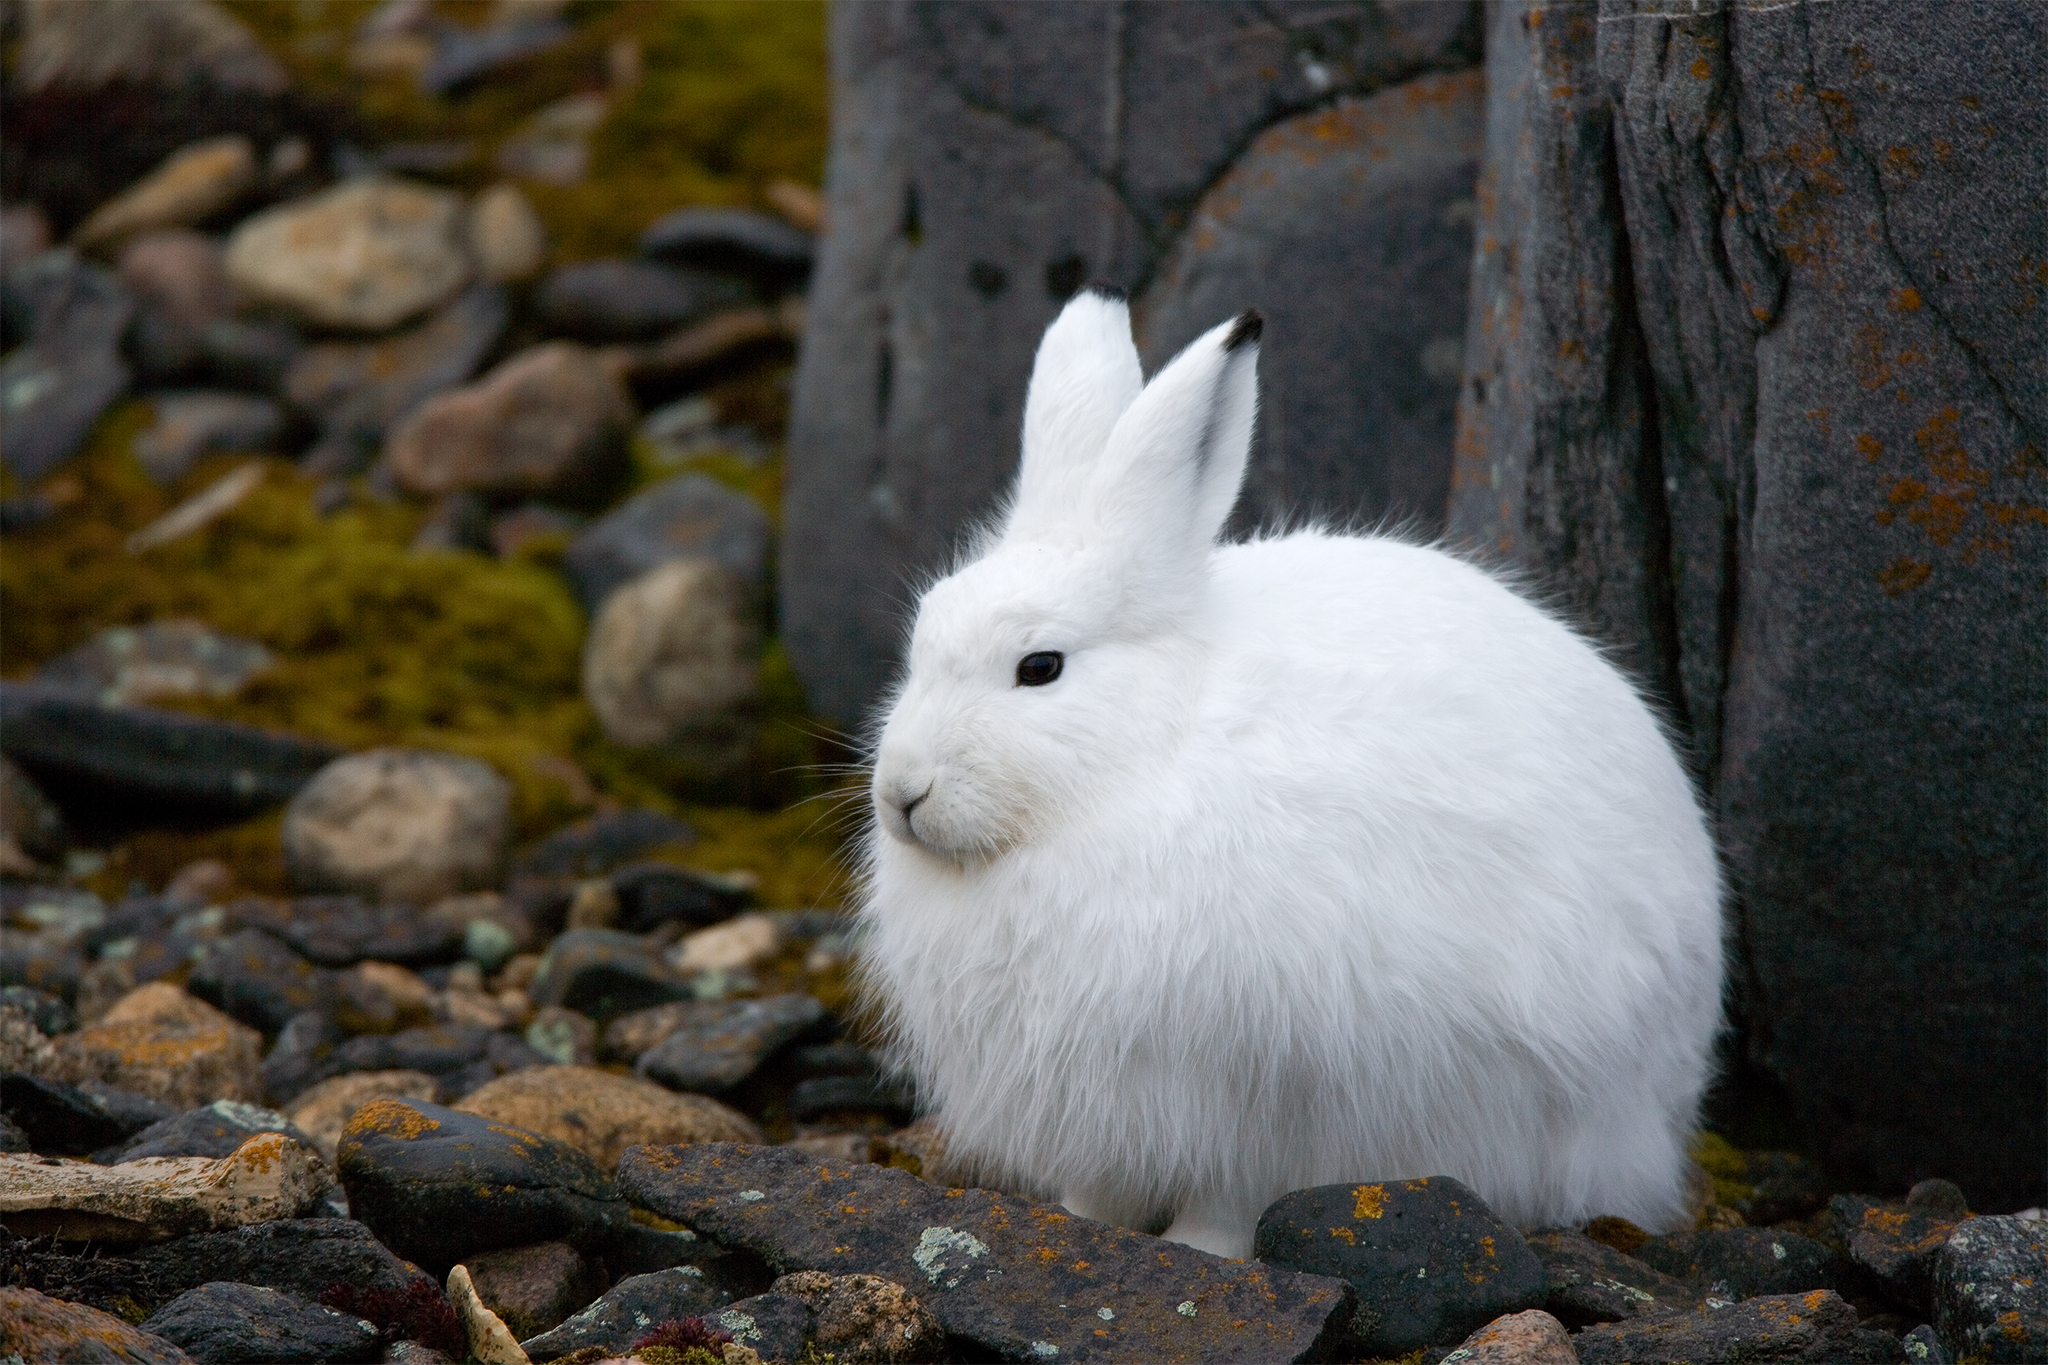
\includegraphics{81736.jpg}
\caption{Image source: National Geographic}
\end{figure}

All of your organized and well-annotated code (with warnings/messages
hidden) used to create at least:

One finalized graph about the Bonanza Creek snowshoe hare population
(you pick which variables, how you want to wrangle it beforehand, and
which type of visual to create - but make sure it is beautifully
finalized)

One finalized HTML table (probably created using kable \& kableExtra)
containing summary statistics about the snowshoe hares (again, you pick
which variables, and how you want to group/summarize them)

Make sure that both your figure and table appear in your final knitted
document, each with a useful caption. Include text associated with each
to help the audience understand and interpret the results.

\begin{Shaded}
\begin{Highlighting}[]
\KeywordTok{library}\NormalTok{(tidyverse)}
\KeywordTok{library}\NormalTok{(kableExtra)}
\KeywordTok{library}\NormalTok{(janitor)}
\KeywordTok{library}\NormalTok{(lubridate)}
\KeywordTok{library}\NormalTok{(tidyr)}
\KeywordTok{library}\NormalTok{(ggfortify)}
\KeywordTok{library}\NormalTok{(RColorBrewer)}

\NormalTok{hares<-}\StringTok{ }\KeywordTok{read_csv}\NormalTok{(}\StringTok{"showshoe_lter.csv"}\NormalTok{) }

\NormalTok{hares_mf <-}\StringTok{ }\NormalTok{hares }\OperatorTok\StringTok{ }
\StringTok{  }\KeywordTok{mutate}\NormalTok{(}\DataTypeTok{sex =} \KeywordTok{str_to_lower}\NormalTok{(sex)) }\OperatorTok\StringTok{ }\CommentTok{# change all entries in sex column to lower case}
\StringTok{  }\KeywordTok{filter}\NormalTok{(sex }\OperatorTok{==}\StringTok{ "m"} \OperatorTok{|}\StringTok{ }\NormalTok{sex }\OperatorTok{==}\StringTok{ "f"}\NormalTok{) }\OperatorTok\StringTok{ }\CommentTok{# remove all observations with NA or ? in sex}
\StringTok{  }\KeywordTok{mutate}\NormalTok{(}\DataTypeTok{date =} \KeywordTok{mdy}\NormalTok{(date)) }\OperatorTok\StringTok{ }\CommentTok{# change date format}
\StringTok{  }\KeywordTok{mutate}\NormalTok{(}\DataTypeTok{full_date =}\NormalTok{ date) }\OperatorTok\StringTok{ }\CommentTok{# retain date column}
\StringTok{  }\KeywordTok{separate}\NormalTok{(date, }\DataTypeTok{into =} \KeywordTok{c}\NormalTok{(}\StringTok{"year"}\NormalTok{, }\StringTok{"month"}\NormalTok{, }\StringTok{"day"}\NormalTok{)) }\OperatorTok\StringTok{ }\CommentTok{#create new columns with parsed date info}
\StringTok{  }\KeywordTok{mutate}\NormalTok{(}\DataTypeTok{month =} \KeywordTok{as.numeric}\NormalTok{(month)) }\OperatorTok\StringTok{ }
\StringTok{  }\KeywordTok{mutate}\NormalTok{(}\DataTypeTok{season =} \KeywordTok{ifelse}\NormalTok{(month }\OperatorTok\StringTok{ }\KeywordTok{c}\NormalTok{(}\DecValTok{1}\OperatorTok{:}\DecValTok{4}\NormalTok{, }\DecValTok{11}\NormalTok{, }\DecValTok{12}\NormalTok{), }\StringTok{"winter"}\NormalTok{, }\StringTok{"summer"}\NormalTok{)) }\OperatorTok\StringTok{ }\CommentTok{# organize months into "summer" and "winter"}
\StringTok{  }\KeywordTok{mutate}\NormalTok{(}\DataTypeTok{year =} \KeywordTok{as.numeric}\NormalTok{(year))}
  
\CommentTok{# seems like there are a lot more observations in the summer than in the winter so maybe not an interesting thing to use for visualization}

\CommentTok{# explore graph}
\KeywordTok{ggplot}\NormalTok{(}\DataTypeTok{data =}\NormalTok{ hares_mf, }\KeywordTok{aes}\NormalTok{(}\DataTypeTok{x =}\NormalTok{ weight, }\DataTypeTok{y =}\NormalTok{ hindft))}\OperatorTok{+}
\StringTok{  }\KeywordTok{geom_point}\NormalTok{()}\OperatorTok{+}
\StringTok{  }\KeywordTok{facet_wrap}\NormalTok{(}\OperatorTok{~}\NormalTok{sex)}
\end{Highlighting}
\end{Shaded}

\includegraphics{assignment1_ClaireMadden_files/figure-latex/unnamed-chunk-1-1.pdf}

\begin{Shaded}
\begin{Highlighting}[]
\CommentTok{# this is not that interesting to me}
\end{Highlighting}
\end{Shaded}

\begin{Shaded}
\begin{Highlighting}[]
\CommentTok{# try something else that may be more interesting}

\NormalTok{hares_hist <-}\StringTok{ }\KeywordTok{ggplot}\NormalTok{(}\DataTypeTok{data =}\NormalTok{ hares_mf, }\KeywordTok{aes}\NormalTok{(}\DataTypeTok{x =}\NormalTok{ year))}\OperatorTok{+}
\StringTok{  }\KeywordTok{geom_bar}\NormalTok{(}\KeywordTok{aes}\NormalTok{(}\DataTypeTok{fill =}\NormalTok{ sex), }\DataTypeTok{position =} \StringTok{"dodge"}\NormalTok{)}\OperatorTok{+}
\StringTok{  }\KeywordTok{scale_fill_manual}\NormalTok{(}\DataTypeTok{values =} \KeywordTok{c}\NormalTok{(}\StringTok{"peru"}\NormalTok{, }\StringTok{"peachpuff2"}\NormalTok{), }\DataTypeTok{labels =} \KeywordTok{c}\NormalTok{(}\StringTok{"Female"}\NormalTok{, }\StringTok{"Male"}\NormalTok{))}\OperatorTok{+}
\StringTok{  }\KeywordTok{scale_x_continuous}\NormalTok{(}\DataTypeTok{expand =} \KeywordTok{c}\NormalTok{(}\DecValTok{0}\NormalTok{,}\DecValTok{0}\NormalTok{),}
                     \DataTypeTok{breaks =} \KeywordTok{seq}\NormalTok{(}\DecValTok{1998}\NormalTok{, }\DecValTok{2012}\NormalTok{, }\DecValTok{1}\NormalTok{))}\OperatorTok{+}
\StringTok{  }\KeywordTok{theme_minimal}\NormalTok{()}\OperatorTok{+}
\StringTok{  }\KeywordTok{labs}\NormalTok{(}\DataTypeTok{x =} \StringTok{"Year of Observation"}\NormalTok{,}
       \DataTypeTok{y =} \StringTok{"Observation Count"}\NormalTok{)}\OperatorTok{+}
\StringTok{  }\KeywordTok{theme}\NormalTok{(}\DataTypeTok{legend.title =} \KeywordTok{element_blank}\NormalTok{())}

\NormalTok{hares_hist}
\end{Highlighting}
\end{Shaded}

\includegraphics{assignment1_ClaireMadden_files/figure-latex/unnamed-chunk-2-1.pdf}

\textbf{Figure 1. Snowshoe Hare Monitoring Observations in the Bonanza
Creek Experimental Forest Between 1998 - 2012.}\\
Total number of observations of female and male snowshoe hares are
recorded each year during the monitoring period. Data source: Kielland
K., F. S. Chapin, R. W. Ruess. 2017.

\begin{Shaded}
\begin{Highlighting}[]
\CommentTok{# make a summary table for females}
\NormalTok{hare_summary_f <-}\StringTok{ }\NormalTok{hares_mf }\OperatorTok\StringTok{ }
\StringTok{  }\KeywordTok{filter}\NormalTok{(sex }\OperatorTok{==}\StringTok{ "f"}\NormalTok{) }\OperatorTok\StringTok{ }
\StringTok{  }\KeywordTok{drop_na}\NormalTok{(weight, hindft) }\OperatorTok\StringTok{ }\CommentTok{# take out an values to be able to calculate mean}
\StringTok{  }\KeywordTok{group_by}\NormalTok{(year) }\OperatorTok\StringTok{ }\CommentTok{# organize by year and sex}
\StringTok{  }\KeywordTok{summarize}\NormalTok{(}
    \DataTypeTok{count =} \KeywordTok{length}\NormalTok{(sex), }\CommentTok{# number of observations}
    \DataTypeTok{avg_weight =} \KeywordTok{round}\NormalTok{(}\KeywordTok{mean}\NormalTok{(weight), }\DataTypeTok{digits =} \DecValTok{0}\NormalTok{))}\CommentTok{# mean weight}
    
\CommentTok{# make a summary table for males}
\NormalTok{hare_summary_m <-}\StringTok{ }\NormalTok{hares_mf }\OperatorTok\StringTok{ }
\StringTok{  }\KeywordTok{filter}\NormalTok{(sex }\OperatorTok{==}\StringTok{ "m"}\NormalTok{) }\OperatorTok\StringTok{ }
\StringTok{  }\KeywordTok{drop_na}\NormalTok{(weight, hindft) }\OperatorTok\StringTok{ }\CommentTok{# take out an values to be able to calculate mean}
\StringTok{  }\KeywordTok{group_by}\NormalTok{(year) }\OperatorTok\StringTok{ }\CommentTok{# organize by year and sex}
\StringTok{  }\KeywordTok{summarize}\NormalTok{(}
    \DataTypeTok{count =} \KeywordTok{length}\NormalTok{(sex), }\CommentTok{# number of observations}
    \DataTypeTok{avg_weight =} \KeywordTok{round}\NormalTok{(}\KeywordTok{mean}\NormalTok{(weight), }\DataTypeTok{digits =} \DecValTok{0}\NormalTok{)) }\CommentTok{# mean weight}

\CommentTok{# combine the two tables!}
\NormalTok{hare_summary <-}\StringTok{ }\KeywordTok{merge}\NormalTok{(hare_summary_f, hare_summary_m, }\DataTypeTok{by =} \StringTok{"year"}\NormalTok{)}

\CommentTok{# format into a single pretty table}
\NormalTok{hare_table <-}\StringTok{ }\KeywordTok{kable}\NormalTok{(hare_summary, }\DataTypeTok{align =} \StringTok{"c"}\NormalTok{, }\DataTypeTok{col.names =} \KeywordTok{c}\NormalTok{(}\StringTok{"Year"}\NormalTok{, }\StringTok{"Count"}\NormalTok{, }\StringTok{"Average Weight (g)"}\NormalTok{, }\StringTok{"Count"}\NormalTok{, }\StringTok{"Average Weight (g)"}\NormalTok{), }\DataTypeTok{caption =} \StringTok{"Table 1. Sumamry Statistics for Snowshoe Hare Monitoring Observations at Bonanza Creek Experimental Forest Between 1998 - 2012. Annual observation counts and average weight of female and male snowshoe hares are reported for each of the years during the monitoring period"}\NormalTok{) }\OperatorTok\StringTok{ }
\StringTok{  }\KeywordTok{add_header_above}\NormalTok{(}\KeywordTok{c}\NormalTok{(}\StringTok{" "}\NormalTok{ =}\StringTok{ }\DecValTok{1}\NormalTok{, }\StringTok{"Female"}\NormalTok{ =}\StringTok{ }\DecValTok{2}\NormalTok{, }\StringTok{"Male"}\NormalTok{ =}\StringTok{ }\DecValTok{2}\NormalTok{)) }\OperatorTok\StringTok{ }
\StringTok{  }\KeywordTok{kable_styling}\NormalTok{(}\DataTypeTok{bootstrap_options =} \KeywordTok{c}\NormalTok{(}\StringTok{"striped"}\NormalTok{), }\DataTypeTok{full_width =} \OtherTok{FALSE}\NormalTok{)}

\NormalTok{hare_table}
\end{Highlighting}
\end{Shaded}

\begin{table}

\caption{\label{tab:unnamed-chunk-3}Table 1. Sumamry Statistics for Snowshoe Hare Monitoring Observations at Bonanza Creek Experimental Forest Between 1998 - 2012. Annual observation counts and average weight of female and male snowshoe hares are reported for each of the years during the monitoring period}
\centering
\begin{tabular}[t]{c|c|c|c|c}
\hline
\multicolumn{1}{c|}{ } & \multicolumn{2}{c|}{Female} & \multicolumn{2}{c}{Male} \\
\cline{2-3} \cline{4-5}
Year & Count & Average Weight (g) & Count & Average Weight (g)\\
\hline
1998 & 10 & 1746 & 5 & 1678\\
\hline
1999 & 113 & 1335 & 136 & 1241\\
\hline
2000 & 78 & 1517 & 47 & 1302\\
\hline
2001 & 25 & 1482 & 27 & 1420\\
\hline
2002 & 10 & 1014 & 17 & 1301\\
\hline
2003 & 33 & 1206 & 23 & 1223\\
\hline
2004 & 45 & 1536 & 29 & 1372\\
\hline
2005 & 47 & 1162 & 36 & 1297\\
\hline
2006 & 29 & 1283 & 15 & 1443\\
\hline
2007 & 57 & 1412 & 25 & 1190\\
\hline
2008 & 87 & 1331 & 76 & 1360\\
\hline
2009 & 117 & 1281 & 100 & 1325\\
\hline
2010 & 96 & 1299 & 43 & 1350\\
\hline
2011 & 85 & 1339 & 43 & 1400\\
\hline
2012 & 24 & 1291 & 21 & 1331\\
\hline
\end{tabular}
\end{table}

Data source: Kielland K., F. S. Chapin, R. W. Ruess. 2017. Snowshoe hare
physical data in Bonanza Creek Experimental Forest: 1999-Present.
Environmental Data Initiative.
\url{https://doi.org/10.6073/pasta/03dce4856d79b91557d8e6ce2cbcdc14}.

\subsubsection{Task 2.}\label{task-2.}

This dataset, compiled and provided by @zander\_venter on Kaggle, is a
compilation of data aquired through Google Earth Engine
(\url{https://earthengine.google.com/}). The dataset uses publically
available remote sensing data, where most of the data is derived by
calculating the mean for each country at a scale of about 10km. In order
to understand the relationship between different environmental and
climatic variables included in the dataset, a principal components
analysis is provided below to demonstrate directionality of the greatest
source of variance within variables considered. These variables were
chosen to demonstrate the relationship of variance between different
climatic variables included in the dataset.

Takeaways from the principal components analysis: - Elevation and
temperature are negatively correlated - Isothermality and temperature
are positively correlated - Mean annual rain, tree cover, and cloudiness
are all positively correlated - Mean annual rain, tree cover, and
cloudiness are not related to elevation or temperature - Principal
components 1 and 2 explain 75\% of variance in the data

\begin{Shaded}
\begin{Highlighting}[]
\CommentTok{# explore data}

\NormalTok{world_env <-}\StringTok{ }\KeywordTok{read_csv}\NormalTok{(}\StringTok{"world_env_vars.csv"}\NormalTok{) }\OperatorTok\StringTok{ }
\StringTok{  }\KeywordTok{clean_names}\NormalTok{(}\DataTypeTok{case =} \StringTok{"upper_camel"}\NormalTok{)}

\KeywordTok{summary}\NormalTok{(world_env) }\CommentTok{# check out the dataset}
\end{Highlighting}
\end{Shaded}

\begin{Shaded}
\begin{Highlighting}[]
\CommentTok{# select variables of interest for principal components analysis}
\NormalTok{env_subset <-}\StringTok{ }\NormalTok{world_env }\OperatorTok\StringTok{ }
\StringTok{  }\KeywordTok{select}\NormalTok{(Elevation, TreeCanopyCover, Isothermality, RainMeanAnnual, TempMeanAnnual, Cloudiness) }

\CommentTok{# explore missingness}

\NormalTok{VIM}\OperatorTok{::}\KeywordTok{matrixplot}\NormalTok{(env_subset, }\DataTypeTok{sortby =} \StringTok{"Elevation"}\NormalTok{)}
\end{Highlighting}
\end{Shaded}

\includegraphics{assignment1_ClaireMadden_files/figure-latex/unnamed-chunk-5-1.pdf}

\begin{Shaded}
\begin{Highlighting}[]
\CommentTok{# can't see variable names so not that helpful for exploration}

\NormalTok{naniar}\OperatorTok{::}\KeywordTok{gg_miss_var}\NormalTok{(env_subset)}
\end{Highlighting}
\end{Shaded}

\includegraphics{assignment1_ClaireMadden_files/figure-latex/unnamed-chunk-5-2.pdf}

\begin{Shaded}
\begin{Highlighting}[]
\CommentTok{# only a few NAs for each variable, will remove them}

\NormalTok{env_nona <-}\StringTok{ }\NormalTok{env_subset }\OperatorTok\StringTok{ }
\StringTok{  }\KeywordTok{drop_na}\NormalTok{() }\CommentTok{# remove NA values}


\NormalTok{env_pca <-}\StringTok{ }\KeywordTok{prcomp}\NormalTok{(env_nona, }\DataTypeTok{scale =} \OtherTok{TRUE}\NormalTok{) }\CommentTok{# run PCA}

\KeywordTok{plot}\NormalTok{(env_pca)}
\end{Highlighting}
\end{Shaded}

\includegraphics{assignment1_ClaireMadden_files/figure-latex/unnamed-chunk-5-3.pdf}

\begin{Shaded}
\begin{Highlighting}[]
\KeywordTok{biplot}\NormalTok{(env_pca) }\CommentTok{# lookin real UGLY! }
\end{Highlighting}
\end{Shaded}

\includegraphics{assignment1_ClaireMadden_files/figure-latex/unnamed-chunk-5-4.pdf}

\begin{Shaded}
\begin{Highlighting}[]
\CommentTok{# a prettier version...}
\NormalTok{my_pca_plot <-}\StringTok{ }\KeywordTok{autoplot}\NormalTok{(env_pca,}
                        \DataTypeTok{colour =} \OtherTok{NA}\NormalTok{,}
                        \DataTypeTok{loadings.colour =} \StringTok{"black"}\NormalTok{,}
                        \DataTypeTok{loadings.label =} \OtherTok{TRUE}\NormalTok{,}
                        \DataTypeTok{loadings.label.size =} \DecValTok{3}\NormalTok{,}
                        \DataTypeTok{loadings.label.colour =} \StringTok{"black"}\NormalTok{,}
                        \DataTypeTok{loadings.label.repel =} \OtherTok{TRUE}\NormalTok{)}\OperatorTok{+}
\StringTok{  }\KeywordTok{theme_bw}\NormalTok{()}

\NormalTok{my_pca_plot}
\end{Highlighting}
\end{Shaded}

\includegraphics{assignment1_ClaireMadden_files/figure-latex/unnamed-chunk-6-1.pdf}

\textbf{Figure 2.} Principal components analysis showing the
relationship between variables included in a compilation\\
of Google Earth Engine datasets.\\
Data source: @zander\_venter.

\end{document}
